
\section{Ejercicio 1}
\subsection{Introducción}

El problema a resolver consiste en lograr conectar la mayor cantidad de ciudades con los metros asignados(sin hacer cortes en el cable). La complejidad pedida es $O(n)$, con $n$ la cantidad de ciudades.

\underline{\textbf{Ejemplos}}

Para los ejemplos denotaremos:

\emph{K}, a la cantidad de kilómetros de cable.\\
\emph{L}, a la lista de los kilometrajes de las estaciones en el ramal sin cosiderar el 0.


\begin{enumerate}
\item 
K = 6, L = [6 8 12 15]\\
El algoritmo debería devolver: 3

\item
K = 35, L = [8 14 20 40 45 54 60 67 74 89 99]\\
El algoritmo debería devolver: 6

\item
K = 4, L = [5 13 19 26 35]\\
El algoritmo debería devolver: 0

\end{enumerate}

\subsection{Desarrollo}

Para simplificar los cálculos, construimos un arreglo a partir de los kilometrajes de entrada que contiene la diferencia entre el kilometraje de una ciudad y su inmediata anterior. Esto representará el costo, en kilómetros de cable, de conectar una ciudad con la más próxima.

Consideramos dos indices sobre el arreglo de costos, que denotarán el inicio y fin de una ruta.
Mientras podemos agregar ciudades a esta ruta, las recorremos con el indice fin.
Cuando el cable restante no es suficiente para agregar una nueva ciudad, corremos el indice de inicio la hasta poder agregar una nueva en el otro extremo de la ruta.
Si no fuera posible, habremos corrido el indice de inicio a la misma posición que la de fin, de manera que contamos con todo el cable posible y aun no pudimos conectar la siguiente ciudad. 
En este caso se sigue a partir de la próxima, ya que era imposible conectar las dos anteriores.

Mantenemos la cantidad de ciudades en la ruta a medida que las sacamos o agregamos, y a partir de esto guardamos la mayor cantidad de ciudades conectadas por una ruta. 
Al agregar o restar ciudades consideramos que al conectar la primer ciudad, estamos implícitamente conectándola con la anterior, y análogamente, al sacar la ultima ciudad, desconectamos dos.

\subsection{Correctitud}
Recibimos una secuencia T de ciudades y un cable de M kilómetros. Tenemos que devolver el tamaño de la mayor subsecuencia de ciudades contiguas en T, que tiene la condición de cubrir una longitud menor o igual a M. Llamaremos $C_i$ a la subsecuencia de mayor tamaño con inicio en la ciudad $i$, y \#$C_i$ a la cantidad de ciudades que cubre.

Lograremos obtener la mayor subsecuencia posible recorriendo todas las subsecuencias maximales (que no se les puede agregar otra ciudad sin superar la distancia M) posibles y quedándonos con la de mayor tamaño.

\newpage

El algoritmo construye todos los $C_{i}$ posicionándose en una ciudad y extendiendo el cable hacia adelante lo más que puede. De ésta forma, crea el $C_{i}$ más largo con ciudad inicial en $i$. Ésto significa que todas las ciudades aparecen como el comienzo de $C_{i}$ para algún $i$, salvo las ciudades que sean parte de la ruta maximal que incluye la última ciudad, que denotaremos $C_f$.
Asimismo, en cada paso guarda el máximo entre \#$C_{i}$ y el máximo guardado a partir de las iteraciones anteriores (o 0, si es la primera), que llamaremos \#$C_{max}$.

Por lo tanto, como todas las secuencias maximales fueron consideradas y ninguna tuvo mayor tamaño, \#$C_{max}$ es el tamaño de la subsecuencia mas grande que se puede cubrir con M kilómetros de cable.


\subsection{Complejidad}

Para la construcción del arreglo de costos recorremos linealmente la lista de kilometrajes de entrada, esto tiene una complejidad $O(n)$.
Luego, para la resolución del problema, recorremos este arreglo a lo sumo dos veces, con costo lineal cada una, por lo que la complejidad final del algoritmo queda acotada por $O(n)$.


\subsection{Experimentación}
Consideramos que el mejor caso para este algoritmo se dará cuando no sea necesario mover el indice de inicio y se itere solo una vez sobre la secuencia de entrada una vez construida la secuencia de costos. Por otro lado, el peor caso se dará cuando ambos indices lleguen al final, iterando dos veces sobre la entrada. 
Sin embargo, en los resultados experimentales observamos que el caso aleatorio tuvo mayor tiempo de ejecución. Relacionamos esto a los distintos costos constantes incurridos en cada ciclo.


\begin{figure}[H]
  \centering
  % GNUPLOT: LaTeX picture
\setlength{\unitlength}{0.240900pt}
\ifx\plotpoint\undefined\newsavebox{\plotpoint}\fi
\begin{picture}(1500,900)(0,0)
\sbox{\plotpoint}{\rule[-0.200pt]{0.400pt}{0.400pt}}%
\put(171.0,131.0){\rule[-0.200pt]{4.818pt}{0.400pt}}
\put(151,131){\makebox(0,0)[r]{$0$}}
\put(1419.0,131.0){\rule[-0.200pt]{4.818pt}{0.400pt}}
\put(171.0,313.0){\rule[-0.200pt]{4.818pt}{0.400pt}}
\put(151,313){\makebox(0,0)[r]{$0.05$}}
\put(1419.0,313.0){\rule[-0.200pt]{4.818pt}{0.400pt}}
\put(171.0,495.0){\rule[-0.200pt]{4.818pt}{0.400pt}}
\put(151,495){\makebox(0,0)[r]{$0.1$}}
\put(1419.0,495.0){\rule[-0.200pt]{4.818pt}{0.400pt}}
\put(171.0,677.0){\rule[-0.200pt]{4.818pt}{0.400pt}}
\put(151,677){\makebox(0,0)[r]{$0.15$}}
\put(1419.0,677.0){\rule[-0.200pt]{4.818pt}{0.400pt}}
\put(171.0,859.0){\rule[-0.200pt]{4.818pt}{0.400pt}}
\put(151,859){\makebox(0,0)[r]{$0.2$}}
\put(1419.0,859.0){\rule[-0.200pt]{4.818pt}{0.400pt}}
\put(171.0,131.0){\rule[-0.200pt]{0.400pt}{4.818pt}}
\put(171,90){\makebox(0,0){$100000$}}
\put(171.0,839.0){\rule[-0.200pt]{0.400pt}{4.818pt}}
\put(312.0,131.0){\rule[-0.200pt]{0.400pt}{4.818pt}}
\put(312,90){\makebox(0,0){$200000$}}
\put(312.0,839.0){\rule[-0.200pt]{0.400pt}{4.818pt}}
\put(453.0,131.0){\rule[-0.200pt]{0.400pt}{4.818pt}}
\put(453,90){\makebox(0,0){$300000$}}
\put(453.0,839.0){\rule[-0.200pt]{0.400pt}{4.818pt}}
\put(594.0,131.0){\rule[-0.200pt]{0.400pt}{4.818pt}}
\put(594,90){\makebox(0,0){$400000$}}
\put(594.0,839.0){\rule[-0.200pt]{0.400pt}{4.818pt}}
\put(735.0,131.0){\rule[-0.200pt]{0.400pt}{4.818pt}}
\put(735,90){\makebox(0,0){$500000$}}
\put(735.0,839.0){\rule[-0.200pt]{0.400pt}{4.818pt}}
\put(875.0,131.0){\rule[-0.200pt]{0.400pt}{4.818pt}}
\put(875,90){\makebox(0,0){$600000$}}
\put(875.0,839.0){\rule[-0.200pt]{0.400pt}{4.818pt}}
\put(1016.0,131.0){\rule[-0.200pt]{0.400pt}{4.818pt}}
\put(1016,90){\makebox(0,0){$700000$}}
\put(1016.0,839.0){\rule[-0.200pt]{0.400pt}{4.818pt}}
\put(1157.0,131.0){\rule[-0.200pt]{0.400pt}{4.818pt}}
\put(1157,90){\makebox(0,0){$800000$}}
\put(1157.0,839.0){\rule[-0.200pt]{0.400pt}{4.818pt}}
\put(1298.0,131.0){\rule[-0.200pt]{0.400pt}{4.818pt}}
\put(1298,90){\makebox(0,0){$900000$}}
\put(1298.0,839.0){\rule[-0.200pt]{0.400pt}{4.818pt}}
\put(1439.0,131.0){\rule[-0.200pt]{0.400pt}{4.818pt}}
\put(1439,90){\makebox(0,0){$1\times10^{6}$}}
\put(1439.0,839.0){\rule[-0.200pt]{0.400pt}{4.818pt}}
\put(171.0,131.0){\rule[-0.200pt]{0.400pt}{175.375pt}}
\put(171.0,131.0){\rule[-0.200pt]{305.461pt}{0.400pt}}
\put(1439.0,131.0){\rule[-0.200pt]{0.400pt}{175.375pt}}
\put(171.0,859.0){\rule[-0.200pt]{305.461pt}{0.400pt}}
\put(30,495){\makebox(0,0){\rotatebox{90}{Tiempo}}}
\put(805,29){\makebox(0,0){Cantidad de valores del arreglo}}
\put(1279,818){\makebox(0,0)[r]{Mejor caso}}
\put(1299.0,818.0){\rule[-0.200pt]{24.090pt}{0.400pt}}
\put(171,140){\usebox{\plotpoint}}
\put(171,139.67){\rule{3.132pt}{0.400pt}}
\multiput(171.00,139.17)(6.500,1.000){2}{\rule{1.566pt}{0.400pt}}
\put(197,140.67){\rule{2.891pt}{0.400pt}}
\multiput(197.00,140.17)(6.000,1.000){2}{\rule{1.445pt}{0.400pt}}
\put(184.0,141.0){\rule[-0.200pt]{3.132pt}{0.400pt}}
\put(222,141.67){\rule{3.132pt}{0.400pt}}
\multiput(222.00,141.17)(6.500,1.000){2}{\rule{1.566pt}{0.400pt}}
\put(235,142.67){\rule{3.132pt}{0.400pt}}
\multiput(235.00,142.17)(6.500,1.000){2}{\rule{1.566pt}{0.400pt}}
\put(209.0,142.0){\rule[-0.200pt]{3.132pt}{0.400pt}}
\put(261,143.67){\rule{2.891pt}{0.400pt}}
\multiput(261.00,143.17)(6.000,1.000){2}{\rule{1.445pt}{0.400pt}}
\put(248.0,144.0){\rule[-0.200pt]{3.132pt}{0.400pt}}
\put(286,144.67){\rule{3.132pt}{0.400pt}}
\multiput(286.00,144.17)(6.500,1.000){2}{\rule{1.566pt}{0.400pt}}
\put(273.0,145.0){\rule[-0.200pt]{3.132pt}{0.400pt}}
\put(312,145.67){\rule{3.132pt}{0.400pt}}
\multiput(312.00,145.17)(6.500,1.000){2}{\rule{1.566pt}{0.400pt}}
\put(299.0,146.0){\rule[-0.200pt]{3.132pt}{0.400pt}}
\put(338,146.67){\rule{2.891pt}{0.400pt}}
\multiput(338.00,146.17)(6.000,1.000){2}{\rule{1.445pt}{0.400pt}}
\put(325.0,147.0){\rule[-0.200pt]{3.132pt}{0.400pt}}
\put(363,147.67){\rule{3.132pt}{0.400pt}}
\multiput(363.00,147.17)(6.500,1.000){2}{\rule{1.566pt}{0.400pt}}
\put(376,148.67){\rule{3.132pt}{0.400pt}}
\multiput(376.00,148.17)(6.500,1.000){2}{\rule{1.566pt}{0.400pt}}
\put(350.0,148.0){\rule[-0.200pt]{3.132pt}{0.400pt}}
\put(402,149.67){\rule{2.891pt}{0.400pt}}
\multiput(402.00,149.17)(6.000,1.000){2}{\rule{1.445pt}{0.400pt}}
\put(389.0,150.0){\rule[-0.200pt]{3.132pt}{0.400pt}}
\put(427,150.67){\rule{3.132pt}{0.400pt}}
\multiput(427.00,150.17)(6.500,1.000){2}{\rule{1.566pt}{0.400pt}}
\put(414.0,151.0){\rule[-0.200pt]{3.132pt}{0.400pt}}
\put(453,151.67){\rule{3.132pt}{0.400pt}}
\multiput(453.00,151.17)(6.500,1.000){2}{\rule{1.566pt}{0.400pt}}
\put(440.0,152.0){\rule[-0.200pt]{3.132pt}{0.400pt}}
\put(478,152.67){\rule{3.132pt}{0.400pt}}
\multiput(478.00,152.17)(6.500,1.000){2}{\rule{1.566pt}{0.400pt}}
\put(491,153.67){\rule{3.132pt}{0.400pt}}
\multiput(491.00,153.17)(6.500,1.000){2}{\rule{1.566pt}{0.400pt}}
\put(466.0,153.0){\rule[-0.200pt]{2.891pt}{0.400pt}}
\put(517,154.67){\rule{3.132pt}{0.400pt}}
\multiput(517.00,154.17)(6.500,1.000){2}{\rule{1.566pt}{0.400pt}}
\put(504.0,155.0){\rule[-0.200pt]{3.132pt}{0.400pt}}
\put(542,155.67){\rule{3.132pt}{0.400pt}}
\multiput(542.00,155.17)(6.500,1.000){2}{\rule{1.566pt}{0.400pt}}
\put(530.0,156.0){\rule[-0.200pt]{2.891pt}{0.400pt}}
\put(568,156.67){\rule{3.132pt}{0.400pt}}
\multiput(568.00,156.17)(6.500,1.000){2}{\rule{1.566pt}{0.400pt}}
\put(581,157.67){\rule{3.132pt}{0.400pt}}
\multiput(581.00,157.17)(6.500,1.000){2}{\rule{1.566pt}{0.400pt}}
\put(555.0,157.0){\rule[-0.200pt]{3.132pt}{0.400pt}}
\put(606,158.67){\rule{3.132pt}{0.400pt}}
\multiput(606.00,158.17)(6.500,1.000){2}{\rule{1.566pt}{0.400pt}}
\put(594.0,159.0){\rule[-0.200pt]{2.891pt}{0.400pt}}
\put(632,159.67){\rule{3.132pt}{0.400pt}}
\multiput(632.00,159.17)(6.500,1.000){2}{\rule{1.566pt}{0.400pt}}
\put(619.0,160.0){\rule[-0.200pt]{3.132pt}{0.400pt}}
\put(658,160.67){\rule{3.132pt}{0.400pt}}
\multiput(658.00,160.17)(6.500,1.000){2}{\rule{1.566pt}{0.400pt}}
\put(645.0,161.0){\rule[-0.200pt]{3.132pt}{0.400pt}}
\put(683,161.67){\rule{3.132pt}{0.400pt}}
\multiput(683.00,161.17)(6.500,1.000){2}{\rule{1.566pt}{0.400pt}}
\put(696,162.67){\rule{3.132pt}{0.400pt}}
\multiput(696.00,162.17)(6.500,1.000){2}{\rule{1.566pt}{0.400pt}}
\put(671.0,162.0){\rule[-0.200pt]{2.891pt}{0.400pt}}
\put(722,163.67){\rule{3.132pt}{0.400pt}}
\multiput(722.00,163.17)(6.500,1.000){2}{\rule{1.566pt}{0.400pt}}
\put(709.0,164.0){\rule[-0.200pt]{3.132pt}{0.400pt}}
\put(747,164.67){\rule{3.132pt}{0.400pt}}
\multiput(747.00,164.17)(6.500,1.000){2}{\rule{1.566pt}{0.400pt}}
\put(735.0,165.0){\rule[-0.200pt]{2.891pt}{0.400pt}}
\put(773,165.67){\rule{3.132pt}{0.400pt}}
\multiput(773.00,165.17)(6.500,1.000){2}{\rule{1.566pt}{0.400pt}}
\put(786,166.67){\rule{3.132pt}{0.400pt}}
\multiput(786.00,166.17)(6.500,1.000){2}{\rule{1.566pt}{0.400pt}}
\put(760.0,166.0){\rule[-0.200pt]{3.132pt}{0.400pt}}
\put(811,167.67){\rule{3.132pt}{0.400pt}}
\multiput(811.00,167.17)(6.500,1.000){2}{\rule{1.566pt}{0.400pt}}
\put(799.0,168.0){\rule[-0.200pt]{2.891pt}{0.400pt}}
\put(837,168.67){\rule{3.132pt}{0.400pt}}
\multiput(837.00,168.17)(6.500,1.000){2}{\rule{1.566pt}{0.400pt}}
\put(850,169.67){\rule{3.132pt}{0.400pt}}
\multiput(850.00,169.17)(6.500,1.000){2}{\rule{1.566pt}{0.400pt}}
\put(824.0,169.0){\rule[-0.200pt]{3.132pt}{0.400pt}}
\put(875,170.67){\rule{3.132pt}{0.400pt}}
\multiput(875.00,170.17)(6.500,1.000){2}{\rule{1.566pt}{0.400pt}}
\put(863.0,171.0){\rule[-0.200pt]{2.891pt}{0.400pt}}
\put(901,171.67){\rule{3.132pt}{0.400pt}}
\multiput(901.00,171.17)(6.500,1.000){2}{\rule{1.566pt}{0.400pt}}
\put(914,172.67){\rule{3.132pt}{0.400pt}}
\multiput(914.00,172.17)(6.500,1.000){2}{\rule{1.566pt}{0.400pt}}
\put(888.0,172.0){\rule[-0.200pt]{3.132pt}{0.400pt}}
\put(939,173.67){\rule{3.132pt}{0.400pt}}
\multiput(939.00,173.17)(6.500,1.000){2}{\rule{1.566pt}{0.400pt}}
\put(927.0,174.0){\rule[-0.200pt]{2.891pt}{0.400pt}}
\put(965,174.67){\rule{3.132pt}{0.400pt}}
\multiput(965.00,174.17)(6.500,1.000){2}{\rule{1.566pt}{0.400pt}}
\put(978,175.67){\rule{3.132pt}{0.400pt}}
\multiput(978.00,175.17)(6.500,1.000){2}{\rule{1.566pt}{0.400pt}}
\put(952.0,175.0){\rule[-0.200pt]{3.132pt}{0.400pt}}
\put(1004,176.67){\rule{2.891pt}{0.400pt}}
\multiput(1004.00,176.17)(6.000,1.000){2}{\rule{1.445pt}{0.400pt}}
\put(991.0,177.0){\rule[-0.200pt]{3.132pt}{0.400pt}}
\put(1029,177.67){\rule{3.132pt}{0.400pt}}
\multiput(1029.00,177.17)(6.500,1.000){2}{\rule{1.566pt}{0.400pt}}
\put(1042,178.67){\rule{3.132pt}{0.400pt}}
\multiput(1042.00,178.17)(6.500,1.000){2}{\rule{1.566pt}{0.400pt}}
\put(1016.0,178.0){\rule[-0.200pt]{3.132pt}{0.400pt}}
\put(1068,179.67){\rule{2.891pt}{0.400pt}}
\multiput(1068.00,179.17)(6.000,1.000){2}{\rule{1.445pt}{0.400pt}}
\put(1080,180.67){\rule{3.132pt}{0.400pt}}
\multiput(1080.00,180.17)(6.500,1.000){2}{\rule{1.566pt}{0.400pt}}
\put(1055.0,180.0){\rule[-0.200pt]{3.132pt}{0.400pt}}
\put(1106,181.67){\rule{3.132pt}{0.400pt}}
\multiput(1106.00,181.17)(6.500,1.000){2}{\rule{1.566pt}{0.400pt}}
\put(1119,182.67){\rule{3.132pt}{0.400pt}}
\multiput(1119.00,182.17)(6.500,1.000){2}{\rule{1.566pt}{0.400pt}}
\put(1093.0,182.0){\rule[-0.200pt]{3.132pt}{0.400pt}}
\put(1144,183.67){\rule{3.132pt}{0.400pt}}
\multiput(1144.00,183.17)(6.500,1.000){2}{\rule{1.566pt}{0.400pt}}
\put(1157,184.67){\rule{3.132pt}{0.400pt}}
\multiput(1157.00,184.17)(6.500,1.000){2}{\rule{1.566pt}{0.400pt}}
\put(1132.0,184.0){\rule[-0.200pt]{2.891pt}{0.400pt}}
\put(1183,185.67){\rule{3.132pt}{0.400pt}}
\multiput(1183.00,185.17)(6.500,1.000){2}{\rule{1.566pt}{0.400pt}}
\put(1170.0,186.0){\rule[-0.200pt]{3.132pt}{0.400pt}}
\put(1208,186.67){\rule{3.132pt}{0.400pt}}
\multiput(1208.00,186.17)(6.500,1.000){2}{\rule{1.566pt}{0.400pt}}
\put(1221,187.67){\rule{3.132pt}{0.400pt}}
\multiput(1221.00,187.17)(6.500,1.000){2}{\rule{1.566pt}{0.400pt}}
\put(1196.0,187.0){\rule[-0.200pt]{2.891pt}{0.400pt}}
\put(1247,188.67){\rule{3.132pt}{0.400pt}}
\multiput(1247.00,188.17)(6.500,1.000){2}{\rule{1.566pt}{0.400pt}}
\put(1260,189.67){\rule{2.891pt}{0.400pt}}
\multiput(1260.00,189.17)(6.000,1.000){2}{\rule{1.445pt}{0.400pt}}
\put(1272,190.67){\rule{3.132pt}{0.400pt}}
\multiput(1272.00,190.17)(6.500,1.000){2}{\rule{1.566pt}{0.400pt}}
\put(1234.0,189.0){\rule[-0.200pt]{3.132pt}{0.400pt}}
\put(1298,191.67){\rule{3.132pt}{0.400pt}}
\multiput(1298.00,191.17)(6.500,1.000){2}{\rule{1.566pt}{0.400pt}}
\put(1311,192.67){\rule{3.132pt}{0.400pt}}
\multiput(1311.00,192.17)(6.500,1.000){2}{\rule{1.566pt}{0.400pt}}
\put(1285.0,192.0){\rule[-0.200pt]{3.132pt}{0.400pt}}
\put(1337,193.67){\rule{2.891pt}{0.400pt}}
\multiput(1337.00,193.17)(6.000,1.000){2}{\rule{1.445pt}{0.400pt}}
\put(1324.0,194.0){\rule[-0.200pt]{3.132pt}{0.400pt}}
\put(1362,194.67){\rule{3.132pt}{0.400pt}}
\multiput(1362.00,194.17)(6.500,1.000){2}{\rule{1.566pt}{0.400pt}}
\put(1375,195.67){\rule{3.132pt}{0.400pt}}
\multiput(1375.00,195.17)(6.500,1.000){2}{\rule{1.566pt}{0.400pt}}
\put(1349.0,195.0){\rule[-0.200pt]{3.132pt}{0.400pt}}
\put(1401,196.67){\rule{2.891pt}{0.400pt}}
\multiput(1401.00,196.17)(6.000,1.000){2}{\rule{1.445pt}{0.400pt}}
\put(1413,197.67){\rule{3.132pt}{0.400pt}}
\multiput(1413.00,197.17)(6.500,1.000){2}{\rule{1.566pt}{0.400pt}}
\put(1388.0,197.0){\rule[-0.200pt]{3.132pt}{0.400pt}}
\put(1426.0,199.0){\rule[-0.200pt]{3.132pt}{0.400pt}}
\put(1279,777){\makebox(0,0)[r]{Peor caso}}
\multiput(1299,777)(20.756,0.000){5}{\usebox{\plotpoint}}
\put(1399,777){\usebox{\plotpoint}}
\put(171,137){\usebox{\plotpoint}}
\put(171.00,137.00){\usebox{\plotpoint}}
\put(191.72,138.00){\usebox{\plotpoint}}
\put(212.43,139.00){\usebox{\plotpoint}}
\put(233.15,139.86){\usebox{\plotpoint}}
\put(253.87,141.00){\usebox{\plotpoint}}
\put(274.58,142.00){\usebox{\plotpoint}}
\put(295.31,142.72){\usebox{\plotpoint}}
\put(316.04,143.31){\usebox{\plotpoint}}
\put(336.73,144.90){\usebox{\plotpoint}}
\put(357.46,145.57){\usebox{\plotpoint}}
\put(378.20,146.17){\usebox{\plotpoint}}
\put(398.89,147.76){\usebox{\plotpoint}}
\put(419.62,148.43){\usebox{\plotpoint}}
\put(440.35,149.03){\usebox{\plotpoint}}
\put(461.05,150.62){\usebox{\plotpoint}}
\put(481.78,151.29){\usebox{\plotpoint}}
\put(502.51,152.00){\usebox{\plotpoint}}
\put(523.20,153.48){\usebox{\plotpoint}}
\put(543.93,154.15){\usebox{\plotpoint}}
\put(564.66,155.00){\usebox{\plotpoint}}
\put(585.36,156.34){\usebox{\plotpoint}}
\put(606.09,157.01){\usebox{\plotpoint}}
\put(626.81,158.00){\usebox{\plotpoint}}
\put(647.52,159.19){\usebox{\plotpoint}}
\put(668.24,160.00){\usebox{\plotpoint}}
\put(688.96,161.00){\usebox{\plotpoint}}
\put(709.67,162.05){\usebox{\plotpoint}}
\put(730.39,163.00){\usebox{\plotpoint}}
\put(751.10,164.00){\usebox{\plotpoint}}
\put(771.82,164.91){\usebox{\plotpoint}}
\put(792.54,166.00){\usebox{\plotpoint}}
\put(813.25,167.00){\usebox{\plotpoint}}
\put(833.98,167.77){\usebox{\plotpoint}}
\put(854.69,169.00){\usebox{\plotpoint}}
\put(875.40,170.00){\usebox{\plotpoint}}
\put(896.13,170.63){\usebox{\plotpoint}}
\put(916.83,172.00){\usebox{\plotpoint}}
\put(937.55,172.88){\usebox{\plotpoint}}
\put(958.29,173.48){\usebox{\plotpoint}}
\put(979.02,174.08){\usebox{\plotpoint}}
\put(999.71,175.67){\usebox{\plotpoint}}
\put(1020.44,176.34){\usebox{\plotpoint}}
\put(1041.17,177.00){\usebox{\plotpoint}}
\put(1061.87,178.53){\usebox{\plotpoint}}
\put(1082.60,179.20){\usebox{\plotpoint}}
\put(1103.29,180.79){\usebox{\plotpoint}}
\put(1124.03,181.39){\usebox{\plotpoint}}
\put(1144.76,182.06){\usebox{\plotpoint}}
\put(1165.45,183.65){\usebox{\plotpoint}}
\put(1186.18,184.24){\usebox{\plotpoint}}
\put(1206.87,185.91){\usebox{\plotpoint}}
\put(1227.60,186.51){\usebox{\plotpoint}}
\put(1248.34,187.10){\usebox{\plotpoint}}
\put(1269.03,188.75){\usebox{\plotpoint}}
\put(1289.76,189.37){\usebox{\plotpoint}}
\put(1310.49,190.00){\usebox{\plotpoint}}
\put(1331.18,191.55){\usebox{\plotpoint}}
\put(1351.91,192.22){\usebox{\plotpoint}}
\put(1372.64,193.00){\usebox{\plotpoint}}
\put(1393.36,194.00){\usebox{\plotpoint}}
\put(1414.07,195.00){\usebox{\plotpoint}}
\put(1434.80,195.68){\usebox{\plotpoint}}
\put(1439,196){\usebox{\plotpoint}}
\sbox{\plotpoint}{\rule[-0.400pt]{0.800pt}{0.800pt}}%
\sbox{\plotpoint}{\rule[-0.200pt]{0.400pt}{0.400pt}}%
\put(1279,736){\makebox(0,0)[r]{Caso promedio}}
\sbox{\plotpoint}{\rule[-0.400pt]{0.800pt}{0.800pt}}%
\put(1299.0,736.0){\rule[-0.400pt]{24.090pt}{0.800pt}}
\put(171,142){\usebox{\plotpoint}}
\put(197,140.84){\rule{2.891pt}{0.800pt}}
\multiput(197.00,140.34)(6.000,1.000){2}{\rule{1.445pt}{0.800pt}}
\put(171.0,142.0){\rule[-0.400pt]{6.263pt}{0.800pt}}
\put(222,141.84){\rule{3.132pt}{0.800pt}}
\multiput(222.00,141.34)(6.500,1.000){2}{\rule{1.566pt}{0.800pt}}
\put(209.0,143.0){\rule[-0.400pt]{3.132pt}{0.800pt}}
\put(248,142.84){\rule{3.132pt}{0.800pt}}
\multiput(248.00,142.34)(6.500,1.000){2}{\rule{1.566pt}{0.800pt}}
\put(235.0,144.0){\rule[-0.400pt]{3.132pt}{0.800pt}}
\put(273,143.84){\rule{3.132pt}{0.800pt}}
\multiput(273.00,143.34)(6.500,1.000){2}{\rule{1.566pt}{0.800pt}}
\put(286,144.84){\rule{3.132pt}{0.800pt}}
\multiput(286.00,144.34)(6.500,1.000){2}{\rule{1.566pt}{0.800pt}}
\put(261.0,145.0){\rule[-0.400pt]{2.891pt}{0.800pt}}
\put(312,145.84){\rule{3.132pt}{0.800pt}}
\multiput(312.00,145.34)(6.500,1.000){2}{\rule{1.566pt}{0.800pt}}
\put(325,146.84){\rule{3.132pt}{0.800pt}}
\multiput(325.00,146.34)(6.500,1.000){2}{\rule{1.566pt}{0.800pt}}
\put(338,147.84){\rule{2.891pt}{0.800pt}}
\multiput(338.00,147.34)(6.000,1.000){2}{\rule{1.445pt}{0.800pt}}
\put(350,148.84){\rule{3.132pt}{0.800pt}}
\multiput(350.00,148.34)(6.500,1.000){2}{\rule{1.566pt}{0.800pt}}
\put(363,149.84){\rule{3.132pt}{0.800pt}}
\multiput(363.00,149.34)(6.500,1.000){2}{\rule{1.566pt}{0.800pt}}
\put(299.0,147.0){\rule[-0.400pt]{3.132pt}{0.800pt}}
\put(389,150.84){\rule{3.132pt}{0.800pt}}
\multiput(389.00,150.34)(6.500,1.000){2}{\rule{1.566pt}{0.800pt}}
\put(402,151.84){\rule{2.891pt}{0.800pt}}
\multiput(402.00,151.34)(6.000,1.000){2}{\rule{1.445pt}{0.800pt}}
\put(414,152.84){\rule{3.132pt}{0.800pt}}
\multiput(414.00,152.34)(6.500,1.000){2}{\rule{1.566pt}{0.800pt}}
\put(427,153.84){\rule{3.132pt}{0.800pt}}
\multiput(427.00,153.34)(6.500,1.000){2}{\rule{1.566pt}{0.800pt}}
\put(440,154.84){\rule{3.132pt}{0.800pt}}
\multiput(440.00,154.34)(6.500,1.000){2}{\rule{1.566pt}{0.800pt}}
\put(453,155.84){\rule{3.132pt}{0.800pt}}
\multiput(453.00,155.34)(6.500,1.000){2}{\rule{1.566pt}{0.800pt}}
\put(466,156.84){\rule{2.891pt}{0.800pt}}
\multiput(466.00,156.34)(6.000,1.000){2}{\rule{1.445pt}{0.800pt}}
\put(478,157.84){\rule{3.132pt}{0.800pt}}
\multiput(478.00,157.34)(6.500,1.000){2}{\rule{1.566pt}{0.800pt}}
\put(491,158.84){\rule{3.132pt}{0.800pt}}
\multiput(491.00,158.34)(6.500,1.000){2}{\rule{1.566pt}{0.800pt}}
\put(504,159.84){\rule{3.132pt}{0.800pt}}
\multiput(504.00,159.34)(6.500,1.000){2}{\rule{1.566pt}{0.800pt}}
\put(517,160.84){\rule{3.132pt}{0.800pt}}
\multiput(517.00,160.34)(6.500,1.000){2}{\rule{1.566pt}{0.800pt}}
\put(530,161.84){\rule{2.891pt}{0.800pt}}
\multiput(530.00,161.34)(6.000,1.000){2}{\rule{1.445pt}{0.800pt}}
\put(542,162.84){\rule{3.132pt}{0.800pt}}
\multiput(542.00,162.34)(6.500,1.000){2}{\rule{1.566pt}{0.800pt}}
\put(555,163.84){\rule{3.132pt}{0.800pt}}
\multiput(555.00,163.34)(6.500,1.000){2}{\rule{1.566pt}{0.800pt}}
\put(568,164.84){\rule{3.132pt}{0.800pt}}
\multiput(568.00,164.34)(6.500,1.000){2}{\rule{1.566pt}{0.800pt}}
\put(581,165.84){\rule{3.132pt}{0.800pt}}
\multiput(581.00,165.34)(6.500,1.000){2}{\rule{1.566pt}{0.800pt}}
\put(594,166.84){\rule{2.891pt}{0.800pt}}
\multiput(594.00,166.34)(6.000,1.000){2}{\rule{1.445pt}{0.800pt}}
\put(606,167.84){\rule{3.132pt}{0.800pt}}
\multiput(606.00,167.34)(6.500,1.000){2}{\rule{1.566pt}{0.800pt}}
\put(619,168.84){\rule{3.132pt}{0.800pt}}
\multiput(619.00,168.34)(6.500,1.000){2}{\rule{1.566pt}{0.800pt}}
\put(632,169.84){\rule{3.132pt}{0.800pt}}
\multiput(632.00,169.34)(6.500,1.000){2}{\rule{1.566pt}{0.800pt}}
\put(645,170.84){\rule{3.132pt}{0.800pt}}
\multiput(645.00,170.34)(6.500,1.000){2}{\rule{1.566pt}{0.800pt}}
\put(658,171.84){\rule{3.132pt}{0.800pt}}
\multiput(658.00,171.34)(6.500,1.000){2}{\rule{1.566pt}{0.800pt}}
\put(671,172.84){\rule{2.891pt}{0.800pt}}
\multiput(671.00,172.34)(6.000,1.000){2}{\rule{1.445pt}{0.800pt}}
\put(683,173.84){\rule{3.132pt}{0.800pt}}
\multiput(683.00,173.34)(6.500,1.000){2}{\rule{1.566pt}{0.800pt}}
\put(696,174.84){\rule{3.132pt}{0.800pt}}
\multiput(696.00,174.34)(6.500,1.000){2}{\rule{1.566pt}{0.800pt}}
\put(709,175.84){\rule{3.132pt}{0.800pt}}
\multiput(709.00,175.34)(6.500,1.000){2}{\rule{1.566pt}{0.800pt}}
\put(722,176.84){\rule{3.132pt}{0.800pt}}
\multiput(722.00,176.34)(6.500,1.000){2}{\rule{1.566pt}{0.800pt}}
\put(735,177.84){\rule{2.891pt}{0.800pt}}
\multiput(735.00,177.34)(6.000,1.000){2}{\rule{1.445pt}{0.800pt}}
\put(747,178.84){\rule{3.132pt}{0.800pt}}
\multiput(747.00,178.34)(6.500,1.000){2}{\rule{1.566pt}{0.800pt}}
\put(760,179.84){\rule{3.132pt}{0.800pt}}
\multiput(760.00,179.34)(6.500,1.000){2}{\rule{1.566pt}{0.800pt}}
\put(376.0,152.0){\rule[-0.400pt]{3.132pt}{0.800pt}}
\put(786,180.84){\rule{3.132pt}{0.800pt}}
\multiput(786.00,180.34)(6.500,1.000){2}{\rule{1.566pt}{0.800pt}}
\put(799,181.84){\rule{2.891pt}{0.800pt}}
\multiput(799.00,181.34)(6.000,1.000){2}{\rule{1.445pt}{0.800pt}}
\put(811,182.84){\rule{3.132pt}{0.800pt}}
\multiput(811.00,182.34)(6.500,1.000){2}{\rule{1.566pt}{0.800pt}}
\put(824,183.84){\rule{3.132pt}{0.800pt}}
\multiput(824.00,183.34)(6.500,1.000){2}{\rule{1.566pt}{0.800pt}}
\put(837,184.84){\rule{3.132pt}{0.800pt}}
\multiput(837.00,184.34)(6.500,1.000){2}{\rule{1.566pt}{0.800pt}}
\put(850,185.84){\rule{3.132pt}{0.800pt}}
\multiput(850.00,185.34)(6.500,1.000){2}{\rule{1.566pt}{0.800pt}}
\put(863,186.84){\rule{2.891pt}{0.800pt}}
\multiput(863.00,186.34)(6.000,1.000){2}{\rule{1.445pt}{0.800pt}}
\put(773.0,182.0){\rule[-0.400pt]{3.132pt}{0.800pt}}
\put(888,187.84){\rule{3.132pt}{0.800pt}}
\multiput(888.00,187.34)(6.500,1.000){2}{\rule{1.566pt}{0.800pt}}
\put(901,188.84){\rule{3.132pt}{0.800pt}}
\multiput(901.00,188.34)(6.500,1.000){2}{\rule{1.566pt}{0.800pt}}
\put(914,189.84){\rule{3.132pt}{0.800pt}}
\multiput(914.00,189.34)(6.500,1.000){2}{\rule{1.566pt}{0.800pt}}
\put(927,190.84){\rule{2.891pt}{0.800pt}}
\multiput(927.00,190.34)(6.000,1.000){2}{\rule{1.445pt}{0.800pt}}
\put(939,191.84){\rule{3.132pt}{0.800pt}}
\multiput(939.00,191.34)(6.500,1.000){2}{\rule{1.566pt}{0.800pt}}
\put(952,192.84){\rule{3.132pt}{0.800pt}}
\multiput(952.00,192.34)(6.500,1.000){2}{\rule{1.566pt}{0.800pt}}
\put(965,193.84){\rule{3.132pt}{0.800pt}}
\multiput(965.00,193.34)(6.500,1.000){2}{\rule{1.566pt}{0.800pt}}
\put(978,194.84){\rule{3.132pt}{0.800pt}}
\multiput(978.00,194.34)(6.500,1.000){2}{\rule{1.566pt}{0.800pt}}
\put(875.0,189.0){\rule[-0.400pt]{3.132pt}{0.800pt}}
\put(1004,195.84){\rule{2.891pt}{0.800pt}}
\multiput(1004.00,195.34)(6.000,1.000){2}{\rule{1.445pt}{0.800pt}}
\put(1016,196.84){\rule{3.132pt}{0.800pt}}
\multiput(1016.00,196.34)(6.500,1.000){2}{\rule{1.566pt}{0.800pt}}
\put(1029,197.84){\rule{3.132pt}{0.800pt}}
\multiput(1029.00,197.34)(6.500,1.000){2}{\rule{1.566pt}{0.800pt}}
\put(1042,198.84){\rule{3.132pt}{0.800pt}}
\multiput(1042.00,198.34)(6.500,1.000){2}{\rule{1.566pt}{0.800pt}}
\put(1055,199.84){\rule{3.132pt}{0.800pt}}
\multiput(1055.00,199.34)(6.500,1.000){2}{\rule{1.566pt}{0.800pt}}
\put(1068,200.84){\rule{2.891pt}{0.800pt}}
\multiput(1068.00,200.34)(6.000,1.000){2}{\rule{1.445pt}{0.800pt}}
\put(1080,201.84){\rule{3.132pt}{0.800pt}}
\multiput(1080.00,201.34)(6.500,1.000){2}{\rule{1.566pt}{0.800pt}}
\put(1093,202.84){\rule{3.132pt}{0.800pt}}
\multiput(1093.00,202.34)(6.500,1.000){2}{\rule{1.566pt}{0.800pt}}
\put(1106,203.84){\rule{3.132pt}{0.800pt}}
\multiput(1106.00,203.34)(6.500,1.000){2}{\rule{1.566pt}{0.800pt}}
\put(1119,204.84){\rule{3.132pt}{0.800pt}}
\multiput(1119.00,204.34)(6.500,1.000){2}{\rule{1.566pt}{0.800pt}}
\put(991.0,197.0){\rule[-0.400pt]{3.132pt}{0.800pt}}
\put(1144,205.84){\rule{3.132pt}{0.800pt}}
\multiput(1144.00,205.34)(6.500,1.000){2}{\rule{1.566pt}{0.800pt}}
\put(1157,206.84){\rule{3.132pt}{0.800pt}}
\multiput(1157.00,206.34)(6.500,1.000){2}{\rule{1.566pt}{0.800pt}}
\put(1170,207.84){\rule{3.132pt}{0.800pt}}
\multiput(1170.00,207.34)(6.500,1.000){2}{\rule{1.566pt}{0.800pt}}
\put(1183,208.84){\rule{3.132pt}{0.800pt}}
\multiput(1183.00,208.34)(6.500,1.000){2}{\rule{1.566pt}{0.800pt}}
\put(1196,209.84){\rule{2.891pt}{0.800pt}}
\multiput(1196.00,209.34)(6.000,1.000){2}{\rule{1.445pt}{0.800pt}}
\put(1208,210.84){\rule{3.132pt}{0.800pt}}
\multiput(1208.00,210.34)(6.500,1.000){2}{\rule{1.566pt}{0.800pt}}
\put(1221,211.84){\rule{3.132pt}{0.800pt}}
\multiput(1221.00,211.34)(6.500,1.000){2}{\rule{1.566pt}{0.800pt}}
\put(1234,212.84){\rule{3.132pt}{0.800pt}}
\multiput(1234.00,212.34)(6.500,1.000){2}{\rule{1.566pt}{0.800pt}}
\put(1247,213.84){\rule{3.132pt}{0.800pt}}
\multiput(1247.00,213.34)(6.500,1.000){2}{\rule{1.566pt}{0.800pt}}
\put(1260,214.84){\rule{2.891pt}{0.800pt}}
\multiput(1260.00,214.34)(6.000,1.000){2}{\rule{1.445pt}{0.800pt}}
\put(1272,215.84){\rule{3.132pt}{0.800pt}}
\multiput(1272.00,215.34)(6.500,1.000){2}{\rule{1.566pt}{0.800pt}}
\put(1285,216.84){\rule{3.132pt}{0.800pt}}
\multiput(1285.00,216.34)(6.500,1.000){2}{\rule{1.566pt}{0.800pt}}
\put(1298,217.84){\rule{3.132pt}{0.800pt}}
\multiput(1298.00,217.34)(6.500,1.000){2}{\rule{1.566pt}{0.800pt}}
\put(1311,218.84){\rule{3.132pt}{0.800pt}}
\multiput(1311.00,218.34)(6.500,1.000){2}{\rule{1.566pt}{0.800pt}}
\put(1324,220.34){\rule{3.132pt}{0.800pt}}
\multiput(1324.00,219.34)(6.500,2.000){2}{\rule{1.566pt}{0.800pt}}
\put(1337,221.84){\rule{2.891pt}{0.800pt}}
\multiput(1337.00,221.34)(6.000,1.000){2}{\rule{1.445pt}{0.800pt}}
\put(1349,223.34){\rule{3.132pt}{0.800pt}}
\multiput(1349.00,222.34)(6.500,2.000){2}{\rule{1.566pt}{0.800pt}}
\put(1362,224.84){\rule{3.132pt}{0.800pt}}
\multiput(1362.00,224.34)(6.500,1.000){2}{\rule{1.566pt}{0.800pt}}
\put(1375,226.34){\rule{3.132pt}{0.800pt}}
\multiput(1375.00,225.34)(6.500,2.000){2}{\rule{1.566pt}{0.800pt}}
\put(1388,228.34){\rule{3.132pt}{0.800pt}}
\multiput(1388.00,227.34)(6.500,2.000){2}{\rule{1.566pt}{0.800pt}}
\put(1401,230.34){\rule{2.891pt}{0.800pt}}
\multiput(1401.00,229.34)(6.000,2.000){2}{\rule{1.445pt}{0.800pt}}
\put(1413,232.34){\rule{3.132pt}{0.800pt}}
\multiput(1413.00,231.34)(6.500,2.000){2}{\rule{1.566pt}{0.800pt}}
\put(1426,234.84){\rule{3.132pt}{0.800pt}}
\multiput(1426.00,233.34)(6.500,3.000){2}{\rule{1.566pt}{0.800pt}}
\put(1132.0,207.0){\rule[-0.400pt]{2.891pt}{0.800pt}}
\sbox{\plotpoint}{\rule[-0.500pt]{1.000pt}{1.000pt}}%
\sbox{\plotpoint}{\rule[-0.200pt]{0.400pt}{0.400pt}}%
\put(1279,695){\makebox(0,0)[r]{O(n)}}
\sbox{\plotpoint}{\rule[-0.500pt]{1.000pt}{1.000pt}}%
\multiput(1299,695)(20.756,0.000){5}{\usebox{\plotpoint}}
\put(1399,695){\usebox{\plotpoint}}
\put(171,186){\usebox{\plotpoint}}
\put(171.00,186.00){\usebox{\plotpoint}}
\put(190.37,193.45){\usebox{\plotpoint}}
\put(209.94,200.36){\usebox{\plotpoint}}
\put(229.31,207.81){\usebox{\plotpoint}}
\put(248.68,215.26){\usebox{\plotpoint}}
\put(267.98,222.91){\usebox{\plotpoint}}
\put(287.29,230.50){\usebox{\plotpoint}}
\put(306.66,237.95){\usebox{\plotpoint}}
\put(326.04,245.40){\usebox{\plotpoint}}
\put(345.33,253.05){\usebox{\plotpoint}}
\put(364.65,260.63){\usebox{\plotpoint}}
\put(384.02,268.08){\usebox{\plotpoint}}
\put(403.38,275.57){\usebox{\plotpoint}}
\put(422.63,283.32){\usebox{\plotpoint}}
\put(442.00,290.77){\usebox{\plotpoint}}
\put(461.37,298.22){\usebox{\plotpoint}}
\put(480.61,306.00){\usebox{\plotpoint}}
\put(499.98,313.46){\usebox{\plotpoint}}
\put(519.36,320.91){\usebox{\plotpoint}}
\put(538.63,328.60){\usebox{\plotpoint}}
\put(558.04,335.94){\usebox{\plotpoint}}
\put(577.64,342.71){\usebox{\plotpoint}}
\put(596.98,350.24){\usebox{\plotpoint}}
\put(616.26,357.94){\usebox{\plotpoint}}
\put(635.63,365.40){\usebox{\plotpoint}}
\put(655.00,372.85){\usebox{\plotpoint}}
\put(674.33,380.39){\usebox{\plotpoint}}
\put(693.61,388.08){\usebox{\plotpoint}}
\put(712.98,395.53){\usebox{\plotpoint}}
\put(732.35,402.98){\usebox{\plotpoint}}
\put(751.59,410.77){\usebox{\plotpoint}}
\put(770.96,418.22){\usebox{\plotpoint}}
\put(790.34,425.67){\usebox{\plotpoint}}
\put(809.59,433.41){\usebox{\plotpoint}}
\put(828.95,440.90){\usebox{\plotpoint}}
\put(848.32,448.35){\usebox{\plotpoint}}
\put(867.64,455.93){\usebox{\plotpoint}}
\put(886.93,463.59){\usebox{\plotpoint}}
\put(906.43,470.67){\usebox{\plotpoint}}
\put(925.98,477.61){\usebox{\plotpoint}}
\put(945.22,485.39){\usebox{\plotpoint}}
\put(964.59,492.84){\usebox{\plotpoint}}
\put(983.96,500.29){\usebox{\plotpoint}}
\put(1003.33,507.74){\usebox{\plotpoint}}
\put(1022.57,515.53){\usebox{\plotpoint}}
\put(1041.94,522.98){\usebox{\plotpoint}}
\put(1061.32,530.43){\usebox{\plotpoint}}
\put(1080.56,538.21){\usebox{\plotpoint}}
\put(1099.93,545.66){\usebox{\plotpoint}}
\put(1119.30,553.12){\usebox{\plotpoint}}
\put(1138.60,560.75){\usebox{\plotpoint}}
\put(1157.91,568.35){\usebox{\plotpoint}}
\put(1177.28,575.80){\usebox{\plotpoint}}
\put(1196.65,583.27){\usebox{\plotpoint}}
\put(1215.89,591.04){\usebox{\plotpoint}}
\put(1235.27,598.49){\usebox{\plotpoint}}
\put(1254.64,605.94){\usebox{\plotpoint}}
\put(1274.20,612.85){\usebox{\plotpoint}}
\put(1293.58,620.30){\usebox{\plotpoint}}
\put(1312.95,627.75){\usebox{\plotpoint}}
\put(1332.32,635.20){\usebox{\plotpoint}}
\put(1351.56,642.98){\usebox{\plotpoint}}
\put(1370.93,650.43){\usebox{\plotpoint}}
\put(1390.30,657.89){\usebox{\plotpoint}}
\put(1409.58,665.57){\usebox{\plotpoint}}
\put(1428.91,673.12){\usebox{\plotpoint}}
\put(1439,677){\usebox{\plotpoint}}
\sbox{\plotpoint}{\rule[-0.200pt]{0.400pt}{0.400pt}}%
\put(171.0,131.0){\rule[-0.200pt]{0.400pt}{175.375pt}}
\put(171.0,131.0){\rule[-0.200pt]{305.461pt}{0.400pt}}
\put(1439.0,131.0){\rule[-0.200pt]{0.400pt}{175.375pt}}
\put(171.0,859.0){\rule[-0.200pt]{305.461pt}{0.400pt}}
\end{picture}

   %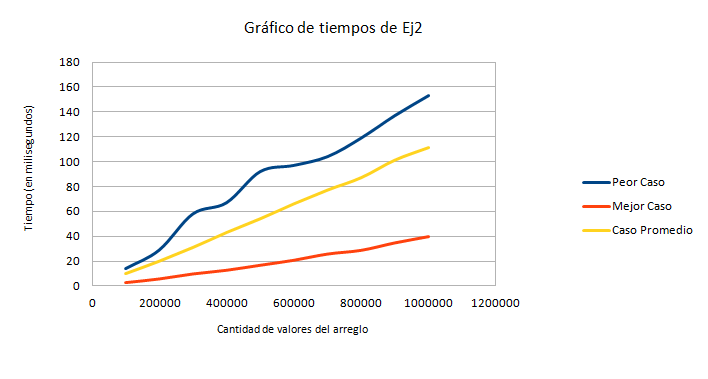
\includegraphics[width=1.1\textwidth]{imagenes/ExperimentoEj2.png}
  \caption{Tiempos de ejecución para ej.1}
\end{figure}

\newpage

Para mostrar el correcto funcionamiento del algoritmo usaremos los siguientes tests, que corren con TelegrafoTestCorrectitud.java.

Caso 1:
Km cable: 10

kilometrajes: 23 55 84 113 140 190 234 302 543

En el primer lugar tenemos un caso donde los kilómetros de cable que se tienen son insuficientes para conectar cualquiera de los puntos.

Caso 2:
Km cable: 1000

kilometrajes: 32 43 65 345 458 679 789 912 934

En este hacemos lo contrario del anterior y le damos suficiente como para conectarlas a todas.

Caso 3:
Km cable: 234

kilometrajes: 2 45 78 90 137 159 563 982 142

En el tercer caso tenemos la cantidad de cable como para llegar a la sexta posición y este nos da la máxima cantidad posible. En otras palabras, nuestro resultado es conectar
las primeras ciudades.

Caso 4:
Km cable: 158

kilometrajes:  451 675 921 1678 2762 2789 2793 2801

Contrario al anterior, conectamos las últimas cuatro.


Caso 5:
Km cable: 19

kilometrajes: 34 59 93 167 192 194 198 254 452

Por último, en vez de conectar las primeras o las segundas, nos queda unido un tramo en la mitad. Osea no las primeras o las últimas sino las que se encuentran en el medio de
la ruta. Y con esto cubrimos todos los hipotéticos casos en cuanto a la ubicación del resultado buscado.









